\chapter*{\iftoggle{german}{Anhang}{Appendix}}
\markboth{}{}
\setcounter{chapter}{1}
\addcontentsline{toc}{chapter}{\iftoggle{german}{Anhang}{Appendix}}

%\DTLloaddb{nodes}{files/data.csv}
%
%This table is automatically generated from a CSV file.
%Of course, you can also create tables from scratch.
%
%\begin{figure}[H]
%    \centering
%    \footnotesize
%    \begin{tabular}{lrrrrrrr} \toprule
%        & \makecell{{List\_}\\{Insert}} & \makecell{{List\_}\\{Search}} & \makecell{{Ordered\_}\\{Insert}} & \makecell{{Ordered\_}\\{Search}} & \makecell{{Ordered\_}\\{Min}} & \makecell{{Ordered\_}\\{Sort}} & \makecell{{Set\_}\\{Insert}}
%        \DTLforeach*{nodes}{\param=Parameter,\listins=ListInsert,\listsea=ListSearch,\ordins=OrderedInsert,\ordsea=OrderedSearch,\ordmin=OrderedMin,\ordsort=OrderedSort,\setins=SetInsert}{
%            \DTLiffirstrow{\\\cmidrule{1-8}}{\\}
%            \param & \listins & \listsea & \ordins & \ordsea & \ordmin & \ordsort & \setins
%        }
%        \\\bottomrule
%    \end{tabular}
%    \caption[Caption in the list of figures]{Caption in the text.}\label{fig:data}
%\end{figure}



\begin{figure}
    \centering
    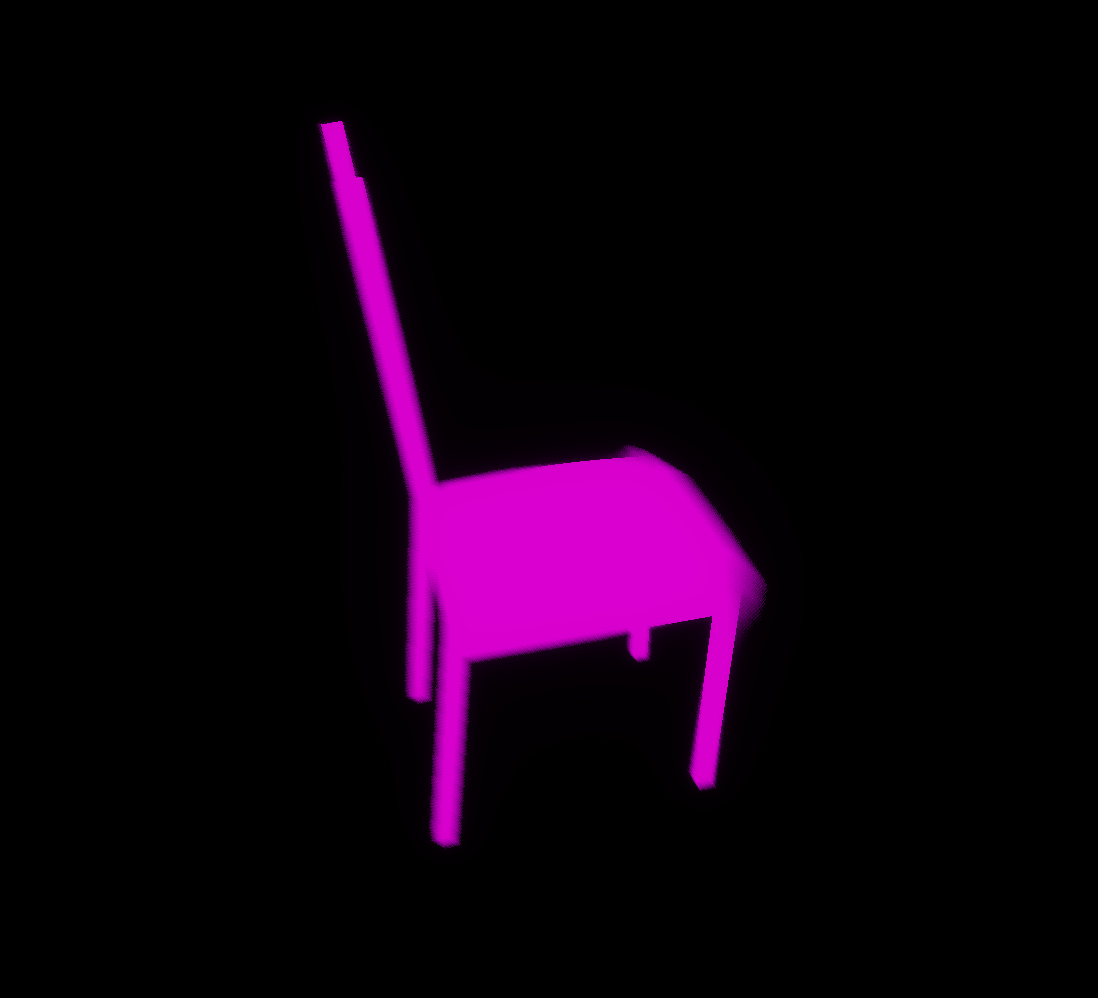
\includegraphics[width=.4\textwidth, height = .3\textwidth]{/Users/apple/OVGU/Thesis/code/3dReconstruction/report/images/appendix/hdrp1}
    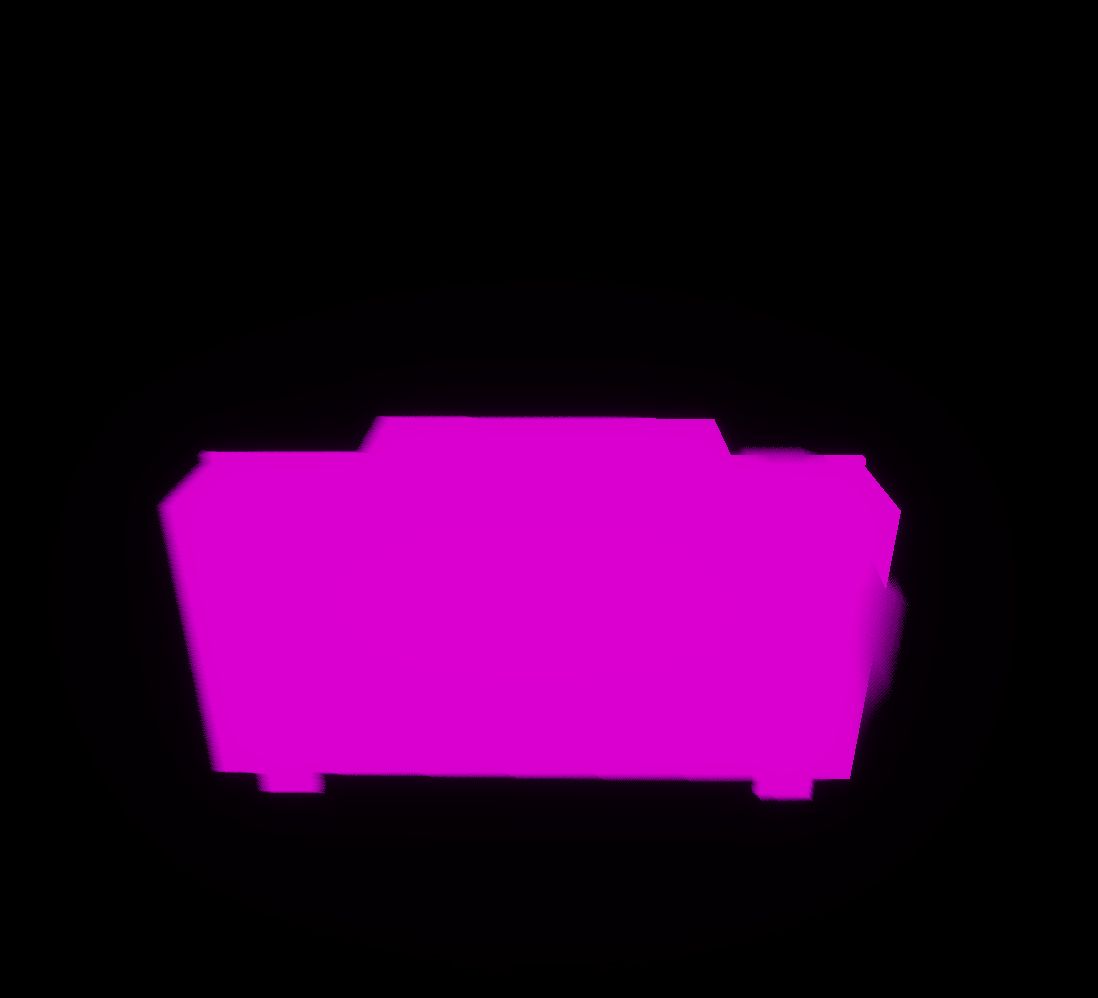
\includegraphics[width=.4\textwidth, height = .3\textwidth,valign=m]{/Users/apple/OVGU/Thesis/code/3dReconstruction/report/images/appendix/hdrp2}\\
    \vspace{0.1cm}
    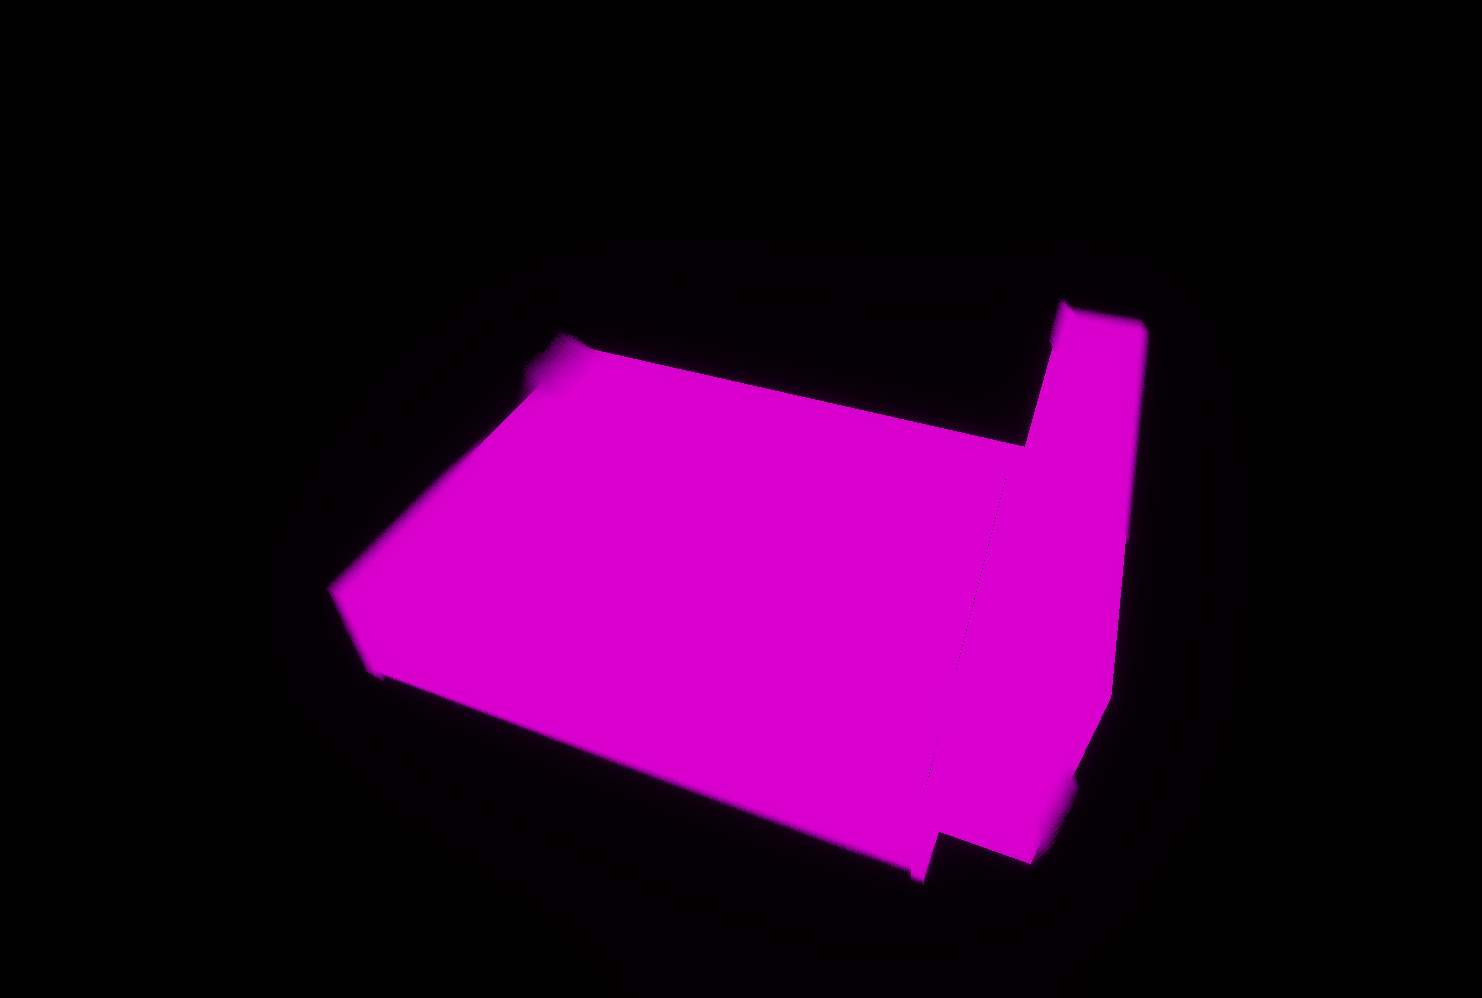
\includegraphics[width=.4\textwidth, height = .3\textwidth]{/Users/apple/OVGU/Thesis/code/3dReconstruction/report/images/appendix/hdrp3}
    
\includegraphics[width=.4\textwidth, height = .3\textwidth]{/Users/apple/OVGU/Thesis/code/3dReconstruction/report/images/appendix/hdrp4}\\
    \caption{Sample images for models rendered in High Definition Render Pipeline of Unity}
    \label{fig:hdrp}
\end{figure}
